\section{Sensorik}
Die Aufgabe der verwendeten Sensorik liegt darin die Werte für $\varphi$, und $\dot{\varphi}$ zu bestimmen. Hierfür wurden zwei MPU6050 IC's verwendet. Diese verfügen jeweils über einen Beschleunigungssensor und Gyroskop, welche Werte für drei Achsen ausgeben. Um die Konfiguration und Auswertung der Sensoren vorzunehmen, bieten diese eine $I^2C$ Schnittstelle an. Die Position und Ausrichtung der Sensoren ist in \ref{Position_Sensoren_pic} dargestellt.

\begin{figure}[h]
\label{Position_Sensoren_pic}
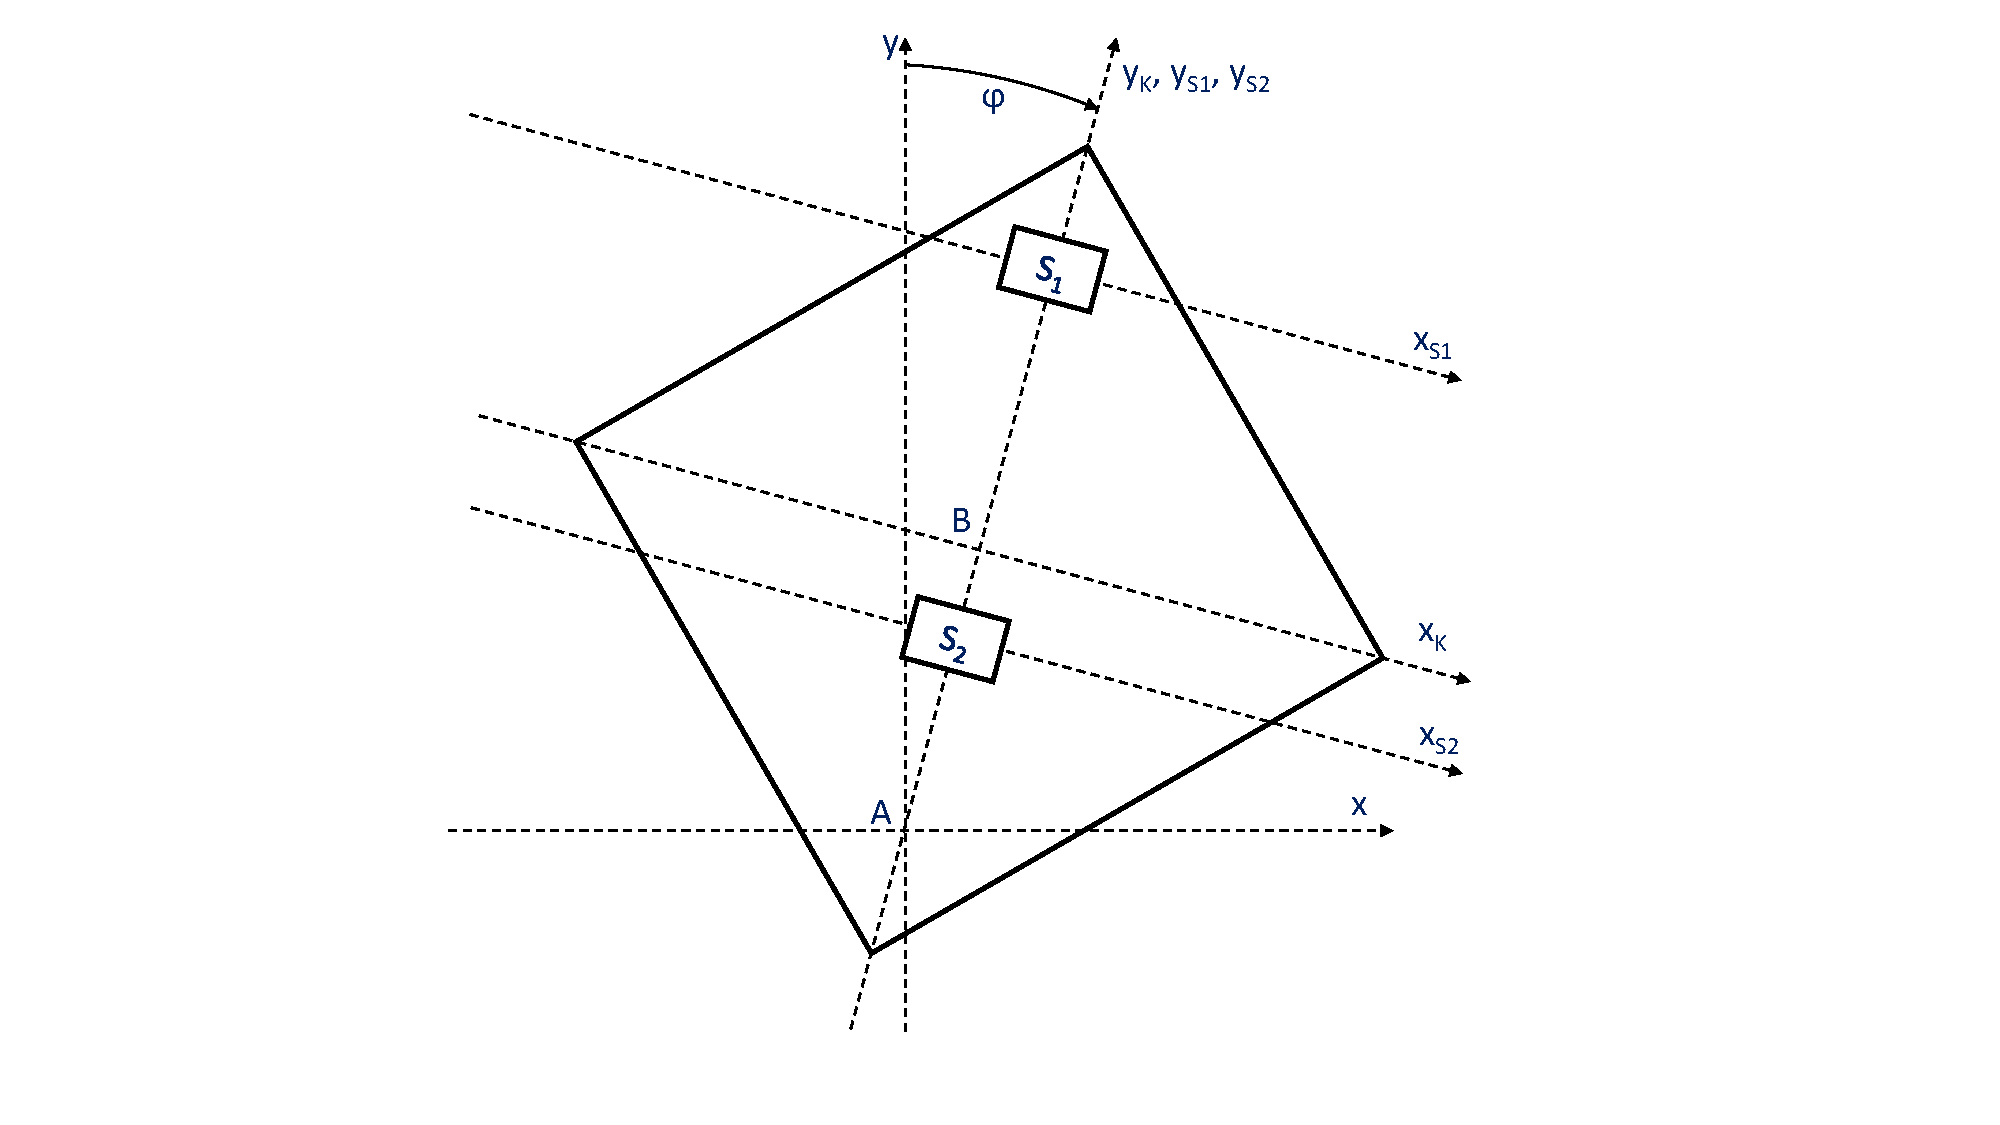
\includegraphics[width=\linewidth]{SensorZeichnung1D}
\caption{Position der Sensoren, Quelle: eigene Darstellung}
\end{figure}

\subsection{Berechnung der Winkelwerte}
Die Sensoren keine Wege bzw. Winkel. Somit muss der Winkel $\varphi$ berechnet werden. Die gemessenen Sensorwerte hängen von $r_{S1}$ bzw. $r_{S2}$ ab, welche den Abstand zwischen den Sensoren und dem Drehpunkt $A$ beschreiben. Zusätzlich beeinflussen neben dem Winkel $\varphi$ auch dessen beiden Ableitungen $\dot{\varphi}$ und $\ddot{\varphi}$ die Sensorausgabe. Allerdings lassen sich aus den Beschleunigungswerten der beiden Sensoren wie folgt der aktuelle Wert von $\varphi$ berechnen.

\begin{equation}
\ddot{S}_i = 
\begin{pmatrix}
\ddot{x}_i \\ \ddot{y}_i \\ \ddot{z}_i
\end{pmatrix} =
\begin{pmatrix}
r_{Si} \cdot \ddot{\varphi} + sin(\varphi) \cdot g \\
- r_{Si} \cdot \dot{\varphi}^2 - cos(\varphi) \cdot g \\
0
\end{pmatrix}
\hspace{35pt}
i \in [1;2]
\end{equation}

\begin{equation}
\alpha = \frac{r_{S1}}{r_{S2}}
\end{equation}

\begin{equation}
\ddot{x}_1 - \alpha \cdot \ddot{x}_2 = 
g(1 - \alpha)sin(\varphi)
\end{equation}
\begin{equation}
\ddot{y}_1 - \alpha \cdot \ddot{y}_2 = 
-g(1- \alpha)cos(\varphi)
\end{equation}

\begin{equation}
\frac{\ddot{x}_1 - \alpha \cdot \ddot{x}_2}{\ddot{y}_1 - \alpha \cdot \ddot{y}_2} = -tan(\varphi)
\end{equation}

